\documentclass[a4paper,12pt]{article}
\usepackage{template}
\addbibresource{biblio.bib}

% Compilation : pdflatex -> bibtex -> pdflatex -> pdflatex
% (ou latexmk -pdf main.tex)

\begin{document}
% Page de titre
\begin{titlepage}
% logos : simples minipages (une figure flottante prendrait le numéro 1)
\noindent
\begin{minipage}{0.35\textwidth}
    
\includegraphics[width=\textwidth]{assets/Logo_Univ_Nantes-optimized.pdf}
\end{minipage}
\hfill
\begin{minipage}{0.35\textwidth}
    
\includegraphics[width=\textwidth]{assets/Logo_Polytech_Nantes_entete-optimized.pdf}
\end{minipage}

\begin{center}
    \vspace*{\fill}
    \normalsize ETN 5 -- Polytech Nantes\\[1mm]
    Langages de description matérielle et réutilisation\\[1.2cm]
    \Large Rapport de mini-projet\\[4mm]
    \LARGE\textbf{Réutilisation de codes HDL\\et HDL réutilisable}\\[1.5cm]
    \large WU Riluke \& LIU Chengpeng\\[1cm]
    \normalsize Enseignant : Sébastien Pillement\\[2mm]
    Octobre 2026
    \vspace*{\fill}
\end{center}
\end{titlepage}


% Sommaire
\tableofcontents
\newpage

\addsec{Introduction}
\markboth{Introduction}{}

\acompleter{objectifs du mini-projet (réutilisation de blocs VHDL, généricité, intégration
d'un processeur RISC-V écrit en Verilog), outils utilisés (ModelSim SE-64 2020.4) et plan du
rapport~\cite{sujet}.}

\clearpage

% Numérotation des parties identique à celle du sujet (parties 2 à 7)
\setcounter{section}{1}
\section{Récupération d'un modèle de RAM}
\label{sec:ram}

Le premier bloc à réutiliser est une RAM synchrone fournie avec son testbench.
Nous avons conservé son fonctionnement, puis adapté les types, les dimensions et la
sélection pour pouvoir relier plusieurs instances au même bus.

\subsection{Analyse du modèle et du testbench}

Le modèle initial, \texttt{ramchip.vhd}, décrit l'entité \texttt{sync\_ram}.
Son adresse de 10 bits donne accès à $2^{10}=1024$ mots de 8 bits. Les entrées sont
l'horloge \texttt{clock}, l'autorisation d'écriture \texttt{we}, l'adresse et la donnée à
écrire ; la sortie \texttt{dataout} fournit la donnée lue. Le tableau mémoire n'est pas
initialisé.

Le code~\ref{lst:ram-originale} distingue deux mécanismes. Au front montant, si
\texttt{we = '1'}, la donnée est écrite à l'adresse présente sur l'entrée. Le même
processus mémorise l'adresse dans \texttt{read\_address}, quelle que soit la valeur de
\texttt{we}. L'affectation concurrente de sortie utilise cette adresse mémorisée : un
changement de l'adresse d'entrée ne suffit donc pas à actualiser la lecture, il faut
attendre le front montant suivant.

\noindent\begin{minipage}{\linewidth}
\begin{lstlisting}[style=vhdl, caption={Lecture et écriture du modèle initial}, label={lst:ram-originale}]
if rising_edge(clock) then
  if we = '1' then
    ram(to_integer(unsigned(address))) <= datain;
  end if;
  read_address <= address;
end if;
...
dataout <= ram(to_integer(unsigned(read_address)));
\end{lstlisting}
\end{minipage}\par

Le fichier \texttt{ram\_tb.vhd} contient deux architectures : \texttt{Bench} présente
un scénario court et \texttt{Bench2} effectue une boucle d'écriture suivie d'une boucle de
lecture. Nous les avons simulées séparément. L'horloge a une période de 10~ns et s'arrête
lorsque \texttt{StopClock} devient vrai.

\paragraph{Scénario court.}
Le testbench modifie ses entrées juste après un front montant, par des affectations de
signaux. Le processus de la RAM voit encore les anciennes valeurs à ce front : les
nouvelles valeurs seront prises en compte au front suivant. Le
tableau~\ref{tab:ram-chrono} donne les principaux événements observés sur la
figure~\ref{fig:ram-originale}.

\begin{table}[H]
\centering
\begin{tabularx}{\linewidth}{rX}
\toprule
Temps & Résultat observé \\
\midrule
25~ns & Écriture de 4 au mot 1 ; la sortie prend la valeur 4 après mise à jour des signaux. \\
35~ns & Écriture de 7 au mot 2 ; la sortie prend la valeur 7. \\
45~ns & Le testbench demande le mot 1 ; l'adresse mémorisée reste 2 et la sortie reste 7. \\
55~ns & L'adresse 1 est mémorisée et la sortie prend la valeur 4. \\
65~ns & L'adresse 2 est mémorisée et la sortie prend la valeur 7. \\
\bottomrule
\end{tabularx}
\caption{Chronologie du test court de la RAM initiale}
\label{tab:ram-chrono}
\end{table}

\simcapture{p2-original.png}{615 564 10 130}{615 154 10 630}
{RAM initiale : écritures de 4 et 7, puis lectures aux adresses 1 et 2}
{fig:ram-originale}

La sortie initiale indéfinie est attendue : ni la mémoire ni le registre d'adresse ne
sont initialisés. ModelSim peut aussi signaler à 0~ns une métavaleur lors de la conversion
de l'adresse en entier. Enfin, quand un front écrit un mot et mémorise en même temps son
adresse, la sortie présente directement la nouvelle donnée : l'affectation concurrente de
sortie est réévaluée après la mise à jour du mot et de l'adresse.

\paragraph{Test en boucle.}
\texttt{Bench2} utilise le signal booléen \texttt{ok}, qui reste faux dès qu'une comparaison
échoue. Notre exécution se termine à 20490~ns avec \texttt{ok = TRUE}. La comparaison
soustrait 1 à l'adresse courante car, au moment où elle est exécutée au front montant,
\texttt{dataout} correspond encore à l'adresse précédente.

Le test a toutefois deux limites : les données se répètent tous les 256 mots, ce qui peut
masquer un défaut sur les bits d'adresse de poids fort, et la dernière donnée lue au mot
1023 n'est pas comparée. Nous avons gardé ce test pour la comparaison avant/après, puis
ajouté un contrôle de toutes les adresses à la section~\ref{sec:ram-generique}.

\subsection{Passage au type unsigned et nouvelle simulation}

Nous avons remplacé \texttt{std\_logic\_vector} par \texttt{unsigned} pour les ports
d'adresse et de données, les mots mémoire, le registre d'adresse et les signaux du
testbench. Ce type de \texttt{numeric\_std} représente un entier non signé et permet
d'écrire directement \texttt{address + 1}.

Les conversions entourant l'adresse deviennent inutiles :
\texttt{to\_integer(unsigned(address))} devient \texttt{to\_integer(address)}.
Le rôle des signaux, leurs largeurs et les conditions de lecture et d'écriture sont
conservés. L'horloge et \texttt{we}, qui ne portent pas des nombres, restent de type
\texttt{std\_logic}.

Nous avons relancé les deux architectures après recompilation. Le scénario court
reproduit les valeurs et les instants du tableau~\ref{tab:ram-chrono}
(figure~\ref{fig:ram-unsigned}). Le test \texttt{Bench2} se termine à nouveau à 20490~ns,
avec \texttt{ok = TRUE}. Ces deux observations confirment la conservation du comportement
pour les scénarios testés.

\simcapture{p2-unsigned.png}{660 564 10 130}{660 154 10 630}
{RAM avec ports unsigned : même chronologie que le modèle initial}
{fig:ram-unsigned}

\subsection{Paramétrage de la capacité et de la largeur des données}
\label{sec:ram-generique}

Deux paramètres \texttt{generic} déterminent les dimensions du bloc
(code~\ref{lst:ram-generique}). \texttt{Nbits\_addr} donne la largeur d'adresse, donc la
capacité vaut $2^{\mathtt{Nbits\_addr}}$ mots ; \texttt{Nbits\_data} donne le nombre de bits
par mot. Nous les avons déclarés de type \texttt{positive} pour exclure les largeurs nulles.
Les valeurs par défaut, 10 et 8, retrouvent le modèle initial.

\noindent\begin{minipage}{\linewidth}
\begin{lstlisting}[style=vhdl, caption={Paramètres et ports de la RAM générique}, label={lst:ram-generique}]
generic (
  Nbits_addr : positive := 10;
  Nbits_data : positive := 8
);
port (
  clock   : in  std_logic;
  we      : in  std_logic;
  address : in  unsigned(Nbits_addr-1 downto 0);
  datain  : in  unsigned(Nbits_data-1 downto 0);
  dataout : out unsigned(Nbits_data-1 downto 0)
);
\end{lstlisting}
\end{minipage}\par

L'architecture utilise déjà les attributs des ports : le tableau contient
\texttt{2**address'length} éléments, chacun de type \texttt{unsigned(datain'range)}, et
\texttt{read\_address} reprend \texttt{address'range}. Elle s'adapte ainsi aux dimensions
choisies sans changer le processus de lecture et d'écriture. Un \texttt{generic map}
permet de choisir une configuration propre à chaque instance.

\paragraph{Vérification de deux configurations.}
Le \texttt{Bench2} hérité compare encore les données à
\texttt{address(7 downto 0) - 1} : il n'est pas adapté à toutes les nouvelles dimensions.
Nous avons donc ajouté l'architecture \texttt{GenericCheck} dans
\path{ram_generic_check.vhd}, en conservant les deux tests précédents.

Ce test écrit puis relit toutes les adresses, y compris la dernière. Les entrées changent
au front descendant, la RAM les échantillonne au front montant et la lecture est contrôlée
au front descendant suivant. Le motif de données replie les bits d'adresse par XOR sur
la largeur du mot ; une seconde passe utilise son complément. Chaque bit de données est
ainsi exercé à 0 et à 1, et tous les bits d'adresse participent au motif. Les deux
configurations du tableau~\ref{tab:ram-generiques} passent ce contrôle.

\begin{table}[H]
\centering
\begin{tabular}{rrrrl}
\toprule
Bits d'adresse & Bits de données & Mots & Fin de simulation & Résultat \\
\midrule
4 & 16 & 16 & 660~ns & \texttt{ok = TRUE} \\
10 & 32 & 1024 & 40980~ns & \texttt{ok = TRUE} \\
\bottomrule
\end{tabular}
\caption{Configurations vérifiées avec deux passes complémentaires}
\label{tab:ram-generiques}
\end{table}

Le modèle de RAM et le testbench sont identiques pour les deux essais ; seuls les
paramètres changent au chargement dans ModelSim. Le contrôle se termine respectivement
à 650 et 40970~ns, puis l'horloge s'arrête une période plus tard. La
figure~\ref{fig:ram-g32} montre les deux passes pour la configuration 1024 mots de 32 bits.

\simcapture{p2-generic-1024x32.png}{660 574 10 130}{660 154 10 630}
{Configuration 1024 mots de 32 bits : même testbench et résultat TRUE}
{fig:ram-g32}

\subsection{Ajout d'une sélection asynchrone CS}

Pour relier plusieurs sorties mémoire, une seule RAM doit piloter le bus à un instant
donné. Nous avons ajouté l'entrée \texttt{cs}, active à 1. Une
affectation concurrente impose la haute impédance lorsque la RAM n'est pas sélectionnée
(code~\ref{lst:ram-cs}). La réaction à \texttt{cs} est asynchrone : elle n'attend pas
de front d'horloge. L'adresse de lecture reste, elle, mémorisée au front montant.

\noindent\begin{minipage}{\linewidth}
\begin{lstlisting}[style=vhdl, caption={Sélection des écritures et commande de la sortie}, label={lst:ram-cs}]
if rising_edge(clock) then
  if we = '1' and cs = '1' then
    ram(to_integer(address)) <= datain;
  end if;
  read_address <= address;
end if;
...
dataout <= ram(to_integer(read_address))
           when cs = '1' else (others => 'Z');
\end{lstlisting}
\end{minipage}\par

La sélection doit aussi conditionner l'écriture : avec un \texttt{we} commun, les RAM
non sélectionnées seraient sinon modifiées. Les essais de la RAM avec sélection et de
\texttt{quadram} ont été relancés après la correction décrite en
section~\ref{sec:validsysteme}.

Le scénario court conserve d'abord les écritures de 4 et 7, puis désactive \texttt{cs}
à 67~ns, entre deux fronts d'horloge. La sortie passe immédiatement en haute impédance.
Au front montant de 85~ns, \texttt{we} vaut 1 et la donnée proposée est 9 à l'adresse 1,
mais \texttt{cs} vaut 0 : le mot reste égal à 4. À 87~ns, la sélection est rétablie,
toujours entre deux fronts, et la sortie reprend immédiatement la valeur 4
(figure~\ref{fig:ram-cs}). La trace interne \texttt{ram(1)} confirme la conservation du mot.

\simcapture{p2-cs.png}{660 564 10 130}{660 154 10 630}
{CS asynchrone : sortie à haute impédance et écriture bloquée entre 67 et 87 ns}
{fig:ram-cs}

\clearpage
\section{Réutilisation du bloc Sync\_Ram}
\label{sec:quadram}

Nous avons ensuite construit \texttt{quadram}, un bloc qui réunit quatre instances de
\texttt{Sync\_Ram} derrière un décodeur. Les RAM partagent les entrées et le bus de sortie ;
le décodeur doit donc sélectionner une seule instance à partir de l'adresse globale.

\subsection{Décodeur d'adresses}

Pour quatre RAM, deux bits de sélection suffisent. Nous avons utilisé une affectation
\texttt{with ... select} pour produire le code à un seul bit actif du
tableau~\ref{tab:decodeur}. Le décodeur est combinatoire : il n'a ni horloge ni état interne.

\begin{table}[H]
\centering
\begin{tabular}{cll}
\toprule
Entrée \texttt{data\_in} & Sortie \texttt{cs\_out(3 downto 0)} & RAM sélectionnée \\
\midrule
\texttt{00} & \texttt{0001} & RAM 0 \\
\texttt{01} & \texttt{0010} & RAM 1 \\
\texttt{10} & \texttt{0100} & RAM 2 \\
\texttt{11} & \texttt{1000} & RAM 3 \\
autres valeurs & \texttt{0000} & aucune \\
\bottomrule
\end{tabular}
\caption{Décodage des deux bits de sélection}
\label{tab:decodeur}
\end{table}

Le cas \texttt{when others} est nécessaire car les bits peuvent notamment prendre les
valeurs indéfinies \texttt{U} ou \texttt{X}. Une adresse indéterminée ne doit pas activer
une RAM. Le testbench applique successivement \texttt{00}, \texttt{01}, \texttt{10},
\texttt{11}, puis \texttt{XX}, pendant 10~ns chacun, et vérifie les sorties par assertions.
Le chronogramme (figure~\ref{fig:decodeur}) reproduit le tableau ; après 40~ns, l'entrée
\texttt{XX} donne bien \texttt{0000}. Les vérifications se terminent à 50~ns.

\simcapture{p3-decoder.png}{660 644 10 130}{660 154 10 630}
{Décodeur 2 vers 4 : une sélection par adresse valide et aucune sélection pour XX}
{fig:decodeur}

\subsection{Assemblage de quatre RAM}

Le fichier \texttt{quadram.vhd} instancie le décodeur et quatre exemplaires du modèle
\texttt{sync\_ram} avec sélection. Chaque RAM est configurée avec
\texttt{Nbits\_addr = 8} et \texttt{Nbits\_data = 8}, soit 256 mots de 8 bits. L'ensemble
contient donc $4\times256=1024$ mots de 8 bits.

L'adresse globale comporte 10 bits. Les bits 9 et 8 sont appliqués au décodeur ; les
bits 7 à 0 désignent le mot à l'intérieur de la RAM. L'adresse locale, les données à
écrire, \texttt{we} et l'horloge sont communes aux quatre instances. Seul le signal
\texttt{cs(i)} est propre à chaque RAM. Le tableau~\ref{tab:quadram-adresses} donne la
répartition de l'espace d'adressage.

\begin{table}[H]
\centering
\begin{tabular}{cll}
\toprule
RAM & Bits 9--8 & Adresses globales (hexadécimal) \\
\midrule
0 & \texttt{00} & \texttt{000} à \texttt{0FF} \\
1 & \texttt{01} & \texttt{100} à \texttt{1FF} \\
2 & \texttt{10} & \texttt{200} à \texttt{2FF} \\
3 & \texttt{11} & \texttt{300} à \texttt{3FF} \\
\bottomrule
\end{tabular}
\caption{Répartition des adresses entre les quatre RAM de 256 mots}
\label{tab:quadram-adresses}
\end{table}

Les sorties sont reliées au même signal \texttt{dataout}. Dans la simulation VHDL, les
éléments résolus de type \texttt{std\_logic} qui composent les vecteurs \texttt{unsigned}
permettent cette connexion à plusieurs pilotes. La RAM sélectionnée fournit la donnée,
les autres fournissent \texttt{Z}. Deux pilotes imposant des valeurs opposées produiraient
une valeur \texttt{X}, d'où la nécessité de n'activer qu'une seule sortie.

\subsection{Validation de l'ensemble}

Nous avons compilé la RAM corrigée, le décodeur et \texttt{quadram} dans une même
bibliothèque, puis exécuté \texttt{quadram\_tb.vhd}. Le test écrit quatre valeurs différentes
au déplacement local 5, puis relit les quatre adresses (tableau~\ref{tab:quadram-test}).

\begin{table}[H]
\centering
\begin{tabular}{clll}
\toprule
RAM & Adresse globale & Donnée écrite et relue & Sélection \\
\midrule
0 & \texttt{005} & \texttt{11} & \texttt{0001} \\
1 & \texttt{105} & \texttt{22} & \texttt{0010} \\
2 & \texttt{205} & \texttt{33} & \texttt{0100} \\
3 & \texttt{305} & \texttt{44} & \texttt{1000} \\
\bottomrule
\end{tabular}
\caption{Test des quatre RAM ; adresses et données en hexadécimal}
\label{tab:quadram-test}
\end{table}

La figure~\ref{fig:quadram-test} montre les écritures de 10 à 50~ns puis les lectures de
50 à 90~ns. Les assertions ne signalent aucune erreur et le message
\og Fin du test de quadram\fg{} apparaît à 90~ns ; l'horloge s'arrête à 100~ns. Les quatre
valeurs restent distinctes : une écriture dans une RAM n'a pas écrasé le mot de même
déplacement dans les autres. Si l'écriture n'était pas conditionnée par \texttt{cs}, les
quatre mots finiraient tous avec la dernière valeur, \texttt{44}, et les trois premières
comparaisons échoueraient.

\simcapture{p3-quadram.png}{660 674 10 130}{660 339 10 550}
{Quadram fixe : écritures puis lectures indépendantes des quatre RAM}
{fig:quadram-test}

\paragraph{Interprétation du temps de lecture.}
Dans ce test, le déplacement local reste égal à 5 pendant le passage d'une RAM à l'autre.
Le changement des bits de sélection modifie donc la sortie dès que le décodeur change
\texttt{cs} : le mot local 5 est déjà adressé dans chaque RAM. Ce comportement ne signifie
pas que toute lecture est asynchrone. Si le déplacement change aussi, la sortie peut
transitoirement présenter la nouvelle RAM à l'ancienne adresse locale, jusqu'au front
montant suivant. Le processeur devra attendre que cette adresse soit échantillonnée avant
de capturer la donnée (section~\ref{sec:synchro}).

Ces quatre lectures vérifient la sélection et l'indépendance des blocs au déplacement 5 ;
elles ne constituent pas un parcours de toutes les adresses de \texttt{quadram}.

\subsection{Généricité du décodeur et de quadram}

Nous avons rendu le décodeur générique avec \texttt{Nbits\_sel}, le nombre de bits de
sélection. Le décodeur produit $2^{\mathtt{Nbits\_sel}}$ sorties, chacune décrite par une
affectation générée (code~\ref{lst:decodeur-generique}).

\noindent\begin{minipage}{\linewidth}
\begin{lstlisting}[style=vhdl, caption={Décodage générique des signaux de sélection}, label={lst:decodeur-generique}]
GEN_CS: for i in 0 to 2**Nbits_sel-1 generate
  cs_out(i) <= '1' when data_in = i else '0';
end generate GEN_CS;
\end{lstlisting}
\end{minipage}\par

Le bloc \texttt{quadram} reçoit trois paramètres : \texttt{Nbits\_sel},
\texttt{Nbits\_addr} et \texttt{Nbits\_data}, notés ici $s$, $a$ et $d$.
Il contient $N=2^s$ RAM de $2^a$ mots de $d$ bits, soit $2^{s+a}$ mots au total ;
l'adresse globale a $s+a$ bits. Le nombre de RAM est donc une puissance de deux :
cette variante ne couvre pas un nombre arbitraire de blocs.

Les instanciations explicites sont remplacées par le code~\ref{lst:quadram-generate}.
\texttt{generate} crée des instances matérielles parallèles à l'élaboration du modèle,
et non une boucle d'exécution partageant une seule RAM.

\noindent\begin{minipage}{\linewidth}
\begin{lstlisting}[style=vhdl, caption={Instances de RAM créées par for ... generate}, label={lst:quadram-generate}]
RAMS: for i in 0 to 2**Nbits_sel-1 generate
  RAM: entity work.sync_ram(RTL)
    generic map (Nbits_addr => Nbits_addr, Nbits_data => Nbits_data)
    port map (cs => cs(i), clock => clock, we => we,
              address => address(Nbits_addr-1 downto 0),
              datain => datain, dataout => dataout);
end generate RAMS;
\end{lstlisting}
\end{minipage}\par

\paragraph{Validation de deux configurations.}
Le testbench écrit au déplacement 5 de la RAM $i$ la valeur \texttt{0x11} multipliée par $i+1$,
puis vérifie la lecture par assertion. Le tableau~\ref{tab:quadram-configs} présente
les deux configurations testées sans modification des sources.

\begin{table}[H]
\centering
\begin{tabular}{rrrrrl}
\toprule
\makecell{Bits de\\sélection} & \makecell{Bits d'adresse\\locale} &
\makecell{Bits de\\données} & RAM & \makecell{Mots\\par RAM} & Résultat \\
\midrule
3 & 4 & 16 & 8 & 16 & aucune assertion en erreur \\
2 & 10 & 32 & 4 & 1024 & aucune assertion en erreur \\
\bottomrule
\end{tabular}
\caption{Configurations du quadram générique effectivement simulées}
\label{tab:quadram-configs}
\end{table}

Avec huit RAM, les adresses \texttt{05}, \texttt{15}, jusqu'à \texttt{75} relisent
\texttt{0011}, \texttt{0022}, jusqu'à \texttt{0088}. Le test se termine à 170~ns et
l'horloge s'arrête à 180~ns (figure~\ref{fig:quadram-g8}).

\simcapture{p3-generic-8x16x16.png}{660 674 10 130}{660 339 10 550}
{Version générique : huit RAM de 16 mots de 16 bits, test des huit sélections}
{fig:quadram-g8}

La configuration du système final contient quatre RAM de 1024 mots de 32 bits.
L'adresse de 12 bits comprend deux bits de sélection et dix bits d'adresse locale.
Les mots \texttt{005}, \texttt{405}, \texttt{805} et \texttt{C05} relisent respectivement
\texttt{11}, \texttt{22}, \texttt{33} et \texttt{44} sur 32 bits. Les assertions passent,
la simulation s'arrête à 100~ns (figure~\ref{fig:quadram-g4}). La sélection et l'isolation
sont ainsi vérifiées au déplacement utilisé dans les deux configurations.

\simcapture{p3-generic-4x1024x32.png}{660 674 10 130}{660 194 10 690}
{Configuration du système final : quatre RAM de 1024 mots de 32 bits}
{fig:quadram-g4}

\clearpage
\section{Prise en main d'un modèle de processeur}
\label{sec:processeur}

Le processeur fourni sur Madoc (\texttt{riscvproc-2.v}) est un modèle comportemental Verilog qui
implémente une partie du jeu d'instructions RV32I~\cite{riscvspec} : \texttt{add},
\texttt{sub}, \texttt{sll}, \texttt{srl}, \texttt{addi}, \texttt{andi}, \texttt{ori},
\texttt{lw}, \texttt{sw} et \texttt{ebreak}. Il contient une mémoire interne \texttt{memory} de
4096 mots de 32 bits, qui sert à la fois au programme et aux données, ainsi que les 32 registres
\texttt{x0} à \texttt{x31}. Une instruction est exécutée toutes les \texttt{Step} = 10~ns ; le
module \texttt{system} n'a aucun port, c'est un modèle purement simulable.

Le fichier utilise des constructions SystemVerilog (\texttt{localparam int unsigned}) : nous
l'avons renommé avec l'extension \texttt{.sv} et compilé avec \texttt{vlog -sv}. L'instruction
\texttt{ebreak} termine la simulation par \texttt{\$finish} ; nous lançons donc \texttt{vsim}
avec l'option \texttt{-onfinish stop}, qui arrête la simulation sans fermer le design et permet
d'examiner ensuite les registres et la mémoire.

% ---------------------------------------------------------------------------
\subsection{Valider le processeur RISC-V}
\label{sec:validation}

Pour faire exécuter un programme, la mémoire du processeur est initialisée au début de la
simulation à partir d'un fichier texte, avec la tâche système \texttt{\$readmemh} placée dans le
bloc \texttt{initial} du processeur (code~\ref{lst:readmemh}). Le fichier contient un mot de
32 bits en hexadécimal par ligne ; \texttt{@0} donne l'adresse du premier mot et \texttt{//}
introduit un commentaire. Le chemin est relatif au répertoire courant de ModelSim : si le
fichier n'est pas trouvé, ModelSim l'indique par un avertissement, la mémoire reste à
\texttt{X} et le processeur affiche \og erreur : mauvaise valeur dans op-code\fg{} à chaque
instruction.

\noindent\begin{minipage}{\linewidth}
\begin{lstlisting}[style=verilog, caption={Chargement du programme dans la mémoire du processeur}, label={lst:readmemh}]
string progfile;
initial begin
  if (!$value$plusargs("prog=%s", progfile))
    progfile = "test_base.txt";
  $readmemh(progfile, memory);
  // initialize program counter to 0
  pc = 0;
  ...
end
\end{lstlisting}
\end{minipage}\par

Nous avons ajouté l'option \texttt{+prog} pour changer de programme sans recompiler le
processeur. Sans cette option, le processeur du code~\ref{lst:readmemh} charge
\texttt{test\_base.txt} ; la commande \texttt{vsim work.system +prog=instr.txt} lui fait charger
\texttt{instr.txt}.

Le programme de test fourni sur Madoc, \texttt{instr.txt}, contient six instructions suivies
de deux données, 2 et 4, que la directive \texttt{@40} place aux mots 64 et 65 (40 en
hexadécimal). Le tableau~\ref{tab:instr} le décode : à la fin du programme, on attend x1 = 1,
x2 = 6 et la valeur 6 au mot 65.

\begin{table}[H]
\centering
\begin{tabular}{clll}
\toprule
Mot & Contenu & Instruction & Effet attendu \\
\midrule
0  & \texttt{04002083} & \texttt{lw x1, 64(x0)}  & x1 = mot 64 = 2 \\
1  & \texttt{04102103} & \texttt{lw x2, 65(x0)}  & x2 = mot 65 = 4 \\
2  & \texttt{00110133} & \texttt{add x2, x2, x1} & x2 = 6 \\
3  & \texttt{001150b3} & \texttt{srl x1, x2, x1} & x1 = 6 décalé de 2 bits = 1 \\
4  & \texttt{0420a023} & \texttt{sw x2, 64(x1)}  & le mot 64 + x1 = 65 reçoit 6 \\
5  & \texttt{00100073} & \texttt{ebreak}         & fin de la simulation \\
\midrule
64 & \texttt{00000002} & donnée & \\
65 & \texttt{00000004} & donnée & \\
\bottomrule
\end{tabular}
\caption{Programme \texttt{instr.txt}}
\label{tab:instr}
\end{table}

Avec le modèle d'origine, aucun de ces résultats n'est obtenu (tableau~\ref{tab:instr-res} et
figure~\ref{fig:instr}).
Les deux \texttt{lw} lisent le mot 0, c'est-à-dire la première instruction
(\texttt{04002083}), au lieu des mots 64 et 65. L'addition et le décalage portent donc sur ce
code : x2 = \texttt{08004106}, puis x1 = \texttt{01000820}, car le décalage vaut les 5 bits
de poids faible de x1, soit 3. Enfin, \texttt{sw} écrit lui aussi au mot 0 : il écrase la
première instruction du programme, et le mot 65 garde sa valeur initiale, 4. Cette erreur
d'adresse, ainsi que celles révélées par le programme \texttt{test\_base}, nous ont conduits
aux corrections de la section~\ref{sec:corrections}. Après ces corrections, \texttt{instr.txt}
donne les valeurs attendues et la simulation se termine à 70~ns.

\begin{table}[H]
\centering
\begin{tabular}{lrrr}
\toprule
 & Attendu & Modèle d'origine & Après correction \\
\midrule
x1      & 1                 & 16779296 (\texttt{01000820})  & 1 \\
x2      & 6                 & 134234374 (\texttt{08004106}) & 6 \\
mot 0   & \texttt{04002083} & \texttt{08004106}             & \texttt{04002083} \\
mot 65  & 6                 & 4                             & 6 \\
\bottomrule
\end{tabular}
\caption{Résultats de \texttt{instr.txt} avant et après correction du modèle}
\label{tab:instr-res}
\end{table}

% figure flottante : en [H] elle laissait un blanc de 7 cm en bas de page
\begin{figure}[tbp]
\centering
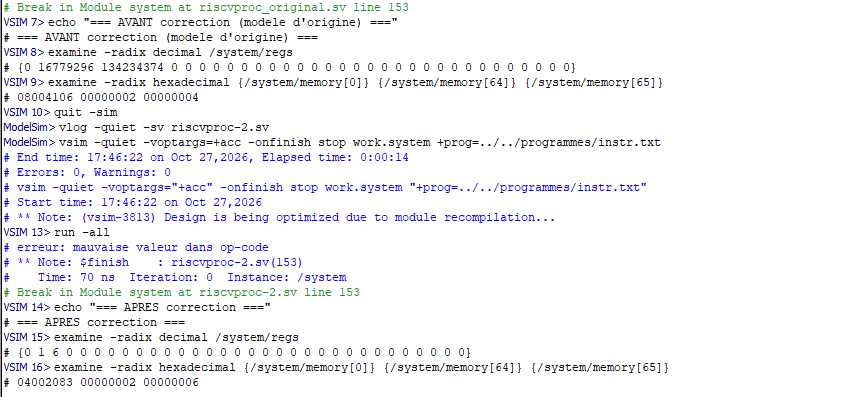
\includegraphics[width=0.98\linewidth]{figures/p4-instr.png}
\caption{Transcript ModelSim : \texttt{instr.txt} avec le modèle d'origine, puis avec le modèle
corrigé}
\label{fig:instr}
\end{figure}

% ---------------------------------------------------------------------------
\subsection{Manipuler les instructions RISC-V (\S\,4.1.1 du sujet)}
\label{sec:codage}

Les instructions RV32I et de l'extension M utilisées ici sont codées sur 32 bits.
Le projet n'utilise pas l'extension C, qui introduit des instructions de 16 bits.
Le modèle utilise trois formats
(tableau~\ref{tab:formats}) : le format R pour les opérations entre registres, le format I pour
les opérations avec un immédiat de 12 bits et pour \texttt{lw}, et le format S pour
\texttt{sw}, dont l'immédiat est découpé en deux champs afin que \texttt{rs1} et \texttt{rs2}
restent à la même place que dans le format R.

\begin{table}[H]
\centering
\begin{tabular}{l|c|c|c|c|c|c|}
\multicolumn{1}{c}{} & \multicolumn{1}{c}{31 -- 25} & \multicolumn{1}{c}{24 -- 20}
 & \multicolumn{1}{c}{19 -- 15} & \multicolumn{1}{c}{14 -- 12} & \multicolumn{1}{c}{11 -- 7}
 & \multicolumn{1}{c}{6 -- 0} \\
\cline{2-7}
R & funct7 & rs2 & rs1 & funct3 & rd & opcode \\
\cline{2-7}
I & \multicolumn{2}{c|}{\texttt{imm[11:0]}} & rs1 & funct3 & rd & opcode \\
\cline{2-7}
S & \texttt{imm[11:5]} & rs2 & rs1 & funct3 & \texttt{imm[4:0]} & opcode \\
\cline{2-7}
\end{tabular}
\caption{Formats d'instructions utilisés (spécification RISC-V, chapitre 2.2)}
\label{tab:formats}
\end{table}

L'instruction \texttt{add x9, x20, x21} est de format R. Ses champs sont donnés dans le
tableau~\ref{tab:add} : le code obtenu est
\texttt{0000 0001 0101 1010 0000 0100 1011 0011}, soit \texttt{0x015A04B3}. L'opcode
\texttt{0110011} désigne les opérations entre registres ; \texttt{funct3} et \texttt{funct7}
choisissent l'opération (\texttt{funct7} vaut \texttt{0100000} pour \texttt{sub}).

\begin{table}[H]
\centering
\begin{tabular}{|c|c|c|c|c|c|}
\hline
funct7 & rs2 = x21 & rs1 = x20 & funct3 & rd = x9 & opcode \\
\hline
\texttt{0000000} & \texttt{10101} & \texttt{10100} & \texttt{000} & \texttt{01001} & \texttt{0110011} \\
\hline
\end{tabular}
\caption{Codage de \texttt{add x9, x20, x21}}
\label{tab:add}
\end{table}

% ---------------------------------------------------------------------------
\subsection{Adapter et implémenter les instructions RISC-V (\S\,4.1.2 du sujet)}
\label{sec:adapter}

\subsubsection{Modes d'adressage}

Le mode d'adressage indique où se trouve l'opérande d'une instruction
(tableau~\ref{tab:adressage}).

\begin{table}[H]
\centering
\begin{tabularx}{\linewidth}{lXl}
\toprule
Mode & Principe & Exemples \\
\midrule
Immédiat & L'opérande est une constante codée dans l'instruction elle-même. & \texttt{addi x1, x0, -7} \\
\addlinespace
Direct & L'adresse mémoire de l'opérande est fixée dans l'instruction ; ici, la base
\texttt{x0} vaut 0. & \texttt{lw x1, 64(x0)} \\
\addlinespace
Indirect & Un registre contient l'adresse de l'opérande en mémoire (pointeur). &
\makecell[tl]{\texttt{lw x1, 0(x2)}\\ \texttt{sw x3, 4(x2)}} \\
\bottomrule
\end{tabularx}
\caption{Modes d'adressage}
\label{tab:adressage}
\end{table}

En RISC-V, \texttt{lw} et \texttt{sw} n'ont qu'un seul mode : l'adresse est la somme d'un
registre de base \texttt{rs1} et d'un déplacement signé de 12 bits, ce qui s'écrit
\texttt{offset(rs1)}. L'adressage direct en est le cas particulier \texttt{rs1} = \texttt{x0} :
\texttt{x0} vaut toujours 0, donc l'adresse 64 de \texttt{lw x1, 64(x0)} est entièrement codée
dans l'instruction. L'adressage indirect en est le cas \texttt{offset} = 0. Dans ce modèle, la
mémoire est adressée par mots de 32 bits (\texttt{memory[addr]}) et non par octets comme dans
la spécification : \texttt{4(x2)} désigne le mot situé 4 mots après l'adresse contenue dans
\texttt{x2}.

\subsubsection{Corrections du modèle fourni}
\label{sec:corrections}

Pour tester les immédiats négatifs, les accès mémoire avec un déplacement positif et négatif,
et le registre \texttt{x0}, nous avons écrit le programme \texttt{test\_base}
(code~\ref{lst:testbase}). Ses résultats sont donnés dans le tableau~\ref{tab:testbase}, relevés
dans ModelSim avec la commande \texttt{examine} (figure~\ref{fig:testbase}) : le modèle d'origine
présente trois erreurs.

\noindent\begin{minipage}{\linewidth}
\begin{lstlisting}[style=code, caption={Programme de test \texttt{test\_base.s}}, label={lst:testbase}]
addi x1, x0, -7      # x1 = -7
addi x2, x0, 100     # x2 = 100
sub  x3, x2, x1      # x3 = 107
andi x4, x1, -16     # x4 = -16
ori  x5, x0, -1      # x5 = -1
addi x6, x0, 3       # x6 = 3
sll  x7, x2, x6      # x7 = 800
srl  x8, x5, x6      # x8 = 0x1FFFFFFF = 536870911
sw   x3, 4(x2)       # mot 104 = 107
sw   x1, -4(x2)      # mot 96 = -7
lw   x9, 4(x2)       # x9 = 107
lw   x10, -4(x2)     # x10 = -7
addi x0, x0, 5       # x0 doit rester a 0
add  x11, x0, x0     # x11 = 0
ebreak
\end{lstlisting}
\end{minipage}\par

\begin{table}[H]
\centering
\begin{tabular}{llrrr}
\toprule
 & Instruction & Attendu & Modèle d'origine & Après correction \\
\midrule
x0  & \texttt{addi x0, x0, 5}   & 0         & 5         & 0 \\
x1  & \texttt{addi x1, x0, -7}  & $-7$      & 4089      & $-7$ \\
x3  & \texttt{sub x3, x2, x1}   & 107       & $-3989$   & 107 \\
x4  & \texttt{andi x4, x1, -16} & $-16$     & 4080      & $-16$ \\
x5  & \texttt{ori x5, x0, -1}   & $-1$      & 4095      & $-1$ \\
x8  & \texttt{srl x8, x5, x6}   & 536870911 & 511       & 536870911 \\
x9  & \texttt{lw x9, 4(x2)}     & 107       & 4089      & 107 \\
x10 & \texttt{lw x10, -4(x2)}   & $-7$      & 4089      & $-7$ \\
x11 & \texttt{add x11, x0, x0}  & 0         & 10        & 0 \\
\midrule
mot 104 & \texttt{sw x3, 4(x2)}  & 107  & \texttt{X} & 107 \\
mot 96  & \texttt{sw x1, -4(x2)} & $-7$ & \texttt{X} & $-7$ \\
mot 0   & première instruction & \texttt{ff900093} & 4089 & \texttt{ff900093} \\
\bottomrule
\end{tabular}
\caption{Résultats de \texttt{test\_base} (x2 = 100, x6 = 3 et x7 = 800 sont corrects dans les deux cas)}
\label{tab:testbase}
\end{table}

\capture[0.8\linewidth]{p4-test-base.png}{Transcript ModelSim, dossier \texttt{exo/p4\_q1} :
\texttt{test\_base} avec le modèle d'origine, puis avec le modèle corrigé}
{Transcript ModelSim : \texttt{test\_base} avec le modèle d'origine, puis avec le modèle
corrigé}{fig:testbase}

Le message \og erreur : mauvaise valeur dans op-code\fg{} affiché au lancement ne vient pas du
programme : ce modèle lit l'instruction par une affectation non bloquante, et l'instruction n'est
pas encore définie à la première période (section~\ref{sec:microarchi}).

\paragraph{Immédiats non étendus en signe.}
Le modèle définissait \lstinline[style=vlinline]|`define I_IMM $signed(instr[31:20])|. Or, en
Verilog, dès qu'un opérande d'une expression est non signé (ici le registre
\texttt{regs[rs1]}), toute l'expression est évaluée en non signé et l'immédiat de 12 bits est
complété par des zéros : $-7$ (\texttt{0xFF9}) devient 4089. C'est l'erreur sur x1, x3, x4 et x5.
Nous faisons l'extension de signe explicitement, en recopiant le bit 31 par concaténation, pour
le format I comme pour le format S (code~\ref{lst:corrections}).

\paragraph{Adresse des accès mémoire.}
L'adresse était calculée par \lstinline[style=vlinline]|addr = `LOAD_OFFSET + regs[`RS1];| avec
\lstinline[style=vlinline]|`define LOAD_OFFSET instr[31:20] << 12|. Une macro est une simple
substitution de texte : la ligne devient
\lstinline[style=vlinline]|addr = instr[31:20] << 12 + regs[`RS1];|, et comme \texttt{+} est
prioritaire sur \lstinline[style=vlinline]|<<|, le déplacement est décalé de 12 + \texttt{rs1} bits. Dans nos
programmes, l'adresse de 12 bits valait donc toujours 0 : les \texttt{lw} lisaient le mot 0 et
les \texttt{sw} écrasaient la première instruction du programme (d'où x9 = x10 = 4089 et le
mot 0 égal à 4089). Le décalage de 12 bits est de toute façon faux : il correspond au format de
\texttt{lui}, pas aux accès mémoire. L'adresse vaut maintenant \texttt{rs1} + immédiat I pour
\texttt{lw}, et \texttt{rs1} + immédiat S pour \texttt{sw}.

\paragraph{Registre x0.}
\texttt{addi x0, x0, 5} modifiait \texttt{x0}, qui doit toujours valoir 0 (spécification,
chapitre 2.1). Nous remettons \texttt{regs[0]} à 0 à la fin de chaque instruction.

\noindent\begin{minipage}{\linewidth}
\begin{lstlisting}[style=verilog, caption={Corrections du modèle (immédiats, adresses, x0)}, label={lst:corrections}]
`define I_IMM   {{20{instr[31]}}, instr[31:20]}               // I-type immediate
`define S_IMM   {{20{instr[31]}}, instr[31:25], instr[11:7]}  // S-type immediate
...
`LW: begin
  addr      = regs[`RS1] + `I_IMM;
  regs[`RD] = memory[addr];
end
...
`SW: begin
  addr         = regs[`RS1] + `S_IMM;
  memory[addr] = regs[`RS2];
end
...
regs[0] = 0;   // x0 is hardwired to 0
\end{lstlisting}
\end{minipage}\par

\subsubsection{Ajout des instructions de l'extension M}
\label{sec:rv32im}

L'extension M ajoute huit instructions de multiplication et de division entières
(tableau~\ref{tab:rv32m}). Ce sont toutes des instructions de format R, avec le même opcode
\texttt{0110011} que \texttt{add} ; elles se distinguent des opérations de RV32I par
\texttt{funct7} = \texttt{0000001} (au lieu de \texttt{0000000} ou \texttt{0100000}), et
\texttt{funct3} choisit l'opération.

\begin{table}[H]
\centering
\begin{tabular}{lcl}
\toprule
Instruction & funct3 & Résultat \\
\midrule
\texttt{MUL}    & \texttt{000} & 32 bits de poids faible de \texttt{rs1} $\times$ \texttt{rs2} \\
\texttt{MULH}   & \texttt{001} & 32 bits de poids fort, signé $\times$ signé \\
\texttt{MULHSU} & \texttt{010} & 32 bits de poids fort, \texttt{rs1} signé $\times$ \texttt{rs2} non signé \\
\texttt{MULHU}  & \texttt{011} & 32 bits de poids fort, non signé $\times$ non signé \\
\texttt{DIV}    & \texttt{100} & quotient signé, arrondi vers 0 \\
\texttt{DIVU}   & \texttt{101} & quotient non signé \\
\texttt{REM}    & \texttt{110} & reste signé, du signe du dividende \\
\texttt{REMU}   & \texttt{111} & reste non signé \\
\bottomrule
\end{tabular}
\caption{Instructions de l'extension M (opcode \texttt{0110011}, funct7 = \texttt{0000001})}
\label{tab:rv32m}
\end{table}

Les modifications à apporter au processeur sont donc les suivantes :
\begin{itemize}
\item \textbf{Décodage} : aucun nouvel opcode n'est nécessaire. Le processeur décode déjà les
opérations entre registres sur le couple \{\texttt{funct3}, \texttt{funct7}\} ; il suffit d'y
ajouter les huit combinaisons.
\item \textbf{Chemin de données} : un multiplieur $32 \times 32$ bits produisant 64 bits, et un
diviseur donnant le quotient et le reste, en versions signée et non signée. Les 32 bits de poids
faible du produit ne dépendent pas du signe des opérandes, d'où une seule instruction
\texttt{MUL} ; les 32 bits de poids fort en dépendent, d'où les trois variantes \texttt{MULH}.
\item \textbf{Cas particuliers} : RISC-V ne déclenche pas d'exception lors d'une division ; la
spécification fixe le résultat de la division par zéro et du dépassement
(tableau~\ref{tab:div0}).
\end{itemize}

\begin{table}[H]
\centering
\begin{tabular}{lcccc}
\toprule
Cas & \texttt{DIV} & \texttt{DIVU} & \texttt{REM} & \texttt{REMU} \\
\midrule
Division par 0 & $-1$ & $2^{32}-1$ & dividende & dividende \\
Dépassement $-2^{31} / (-1)$ & $-2^{31}$ & -- & 0 & -- \\
\bottomrule
\end{tabular}
\caption{Résultats imposés par la spécification pour la division}
\label{tab:div0}
\end{table}

\subsubsection{Implémentation et validation de l'extension M}
\label{sec:rv32im-impl}

Nous avons ajouté les huit codes sous la même forme que les instructions existantes, par exemple
\lstinline[style=vlinline]|`define MUL {3'b000, 7'b0000001}|, et huit cas dans le décodage des
opérations entre registres (code~\ref{lst:rv32m}). Trois points de Verilog demandent de
l'attention :
\begin{itemize}
\item \textbf{Largeur et extension des opérandes.} Dans une affectation directe telle que
\texttt{prod = a * b}, une destination de 64 bits participe au calcul de la largeur de
l'expression : deux opérandes de 32 bits ne provoquent donc pas à eux seuls une troncature
à 32 bits~\cite{systemverilog}. Nos concaténations rendent surtout explicite l'extension
voulue pour chaque opérande : copie du signe avec
\lstinline[style=vlinline]|{{32{x[31]}}, x}| ou ajout de zéros avec
\lstinline[style=vlinline]|{32'b0, x}|. Le produit est conservé sur 64 bits dans
\texttt{prod}, puis les bits 63 à 32 sont copiés pour les variantes \texttt{MULH}.
\item \textbf{Division signée.} Les deux opérandes passent par \texttt{\$signed}. La division
signée de Verilog arrondit vers zéro et le reste prend le signe du dividende, comme en RISC-V.
\item \textbf{Cas particuliers.} En Verilog, une division par zéro donne \texttt{X} ; ces cas sont
donc traités avant la division, avec \texttt{if}/\texttt{else}. Nous avons évité l'opérateur
conditionnel \texttt{? :} : si l'une de ses branches est non signée (par exemple
\texttt{32'hFFFFFFFF}), toute l'expression devient non signée, et la division de l'autre branche
est alors calculée en non signé ($-7 / 2$ donne 2147483644 au lieu de $-3$).
\end{itemize}

\noindent\begin{minipage}{\linewidth}
\begin{lstlisting}[style=verilog, caption={Extrait de l'implémentation de l'extension M}, label={lst:rv32m}]
reg[63:0] prod;   // 64-bit product for MULH, MULHSU, MULHU
...
`MUL:    regs[`RD] = regs[`RS1] * regs[`RS2];  // 32-bit target: low half
`MULH:   begin
           prod = {{32{regs[`RS1][31]}}, regs[`RS1]} * {{32{regs[`RS2][31]}}, regs[`RS2]};
           regs[`RD] = prod[63:32];
         end
...
`DIV:    if (regs[`RS2] == 0)
           regs[`RD] = 32'hFFFFFFFF;                     // division by 0: -1
         else if (regs[`RS1] == 32'h80000000 && regs[`RS2] == 32'hFFFFFFFF)
           regs[`RD] = 32'h80000000;                     // overflow: -2^31
         else
           regs[`RD] = $signed(regs[`RS1]) / $signed(regs[`RS2]);
\end{lstlisting}
\end{minipage}\par

Le programme \texttt{test\_rv32im} teste les huit instructions et les trois cas particuliers.
Avant la modification, le processeur affichait onze fois \og erreur : mauvaise instruction
arithmétique\fg{}, une fois par instruction de l'extension M, et les registres correspondants
restaient à 0 (figure~\ref{fig:rv32im-avant}). Après la modification, toutes les valeurs sont
celles attendues (tableau~\ref{tab:rv32imres} et figure~\ref{fig:rv32im}).

\capture[0.82\linewidth]{p4-rv32im-avant.png}{Transcript ModelSim, dossier \texttt{exo/p4\_q1} :
\texttt{test\_rv32im} avant l'ajout de l'extension M}
{Transcript ModelSim : \texttt{test\_rv32im} avant l'ajout de l'extension M (le transcript
affiche mal l'accent de \og arithmétique\fg{})}{fig:rv32im-avant}

\begin{table}[H]
\centering
\begin{tabular}{llrl}
\toprule
Instruction & Registre & Résultat & Remarque \\
\midrule
\texttt{mul x3, x1, x2}     & x3  & $-14$ & \\
\texttt{div x4, x1, x2}     & x4  & $-3$  & arrondi vers 0 \\
\texttt{rem x5, x1, x2}     & x5  & $-1$  & signe du dividende \\
\texttt{divu x6, x1, x2}    & x6  & 2147483644 & \texttt{0xFFFFFFF9} / 2 \\
\texttt{div x7, x1, x0}     & x7  & $-1$  & division par 0 \\
\texttt{mulh x8, x1, x2}    & x8  & $-1$  & partie haute de $-14$ \\
\texttt{mulhu x9, x1, x2}   & x9  & 1     & \texttt{0xFFFFFFF9} $\times$ 2 = \texttt{0x1FFFFFFF2} \\
\texttt{remu x10, x1, x2}   & x10 & 1     & \\
\texttt{mulhsu x16, x1, x2} & x16 & $-1$  & \\
\texttt{div x14, x11, x12}  & x14 & $-2^{31}$ & dépassement \\
\texttt{rem x15, x11, x12}  & x15 & 0     & dépassement \\
\bottomrule
\end{tabular}
\caption{Résultats de \texttt{test\_rv32im}, avec x1 = $-7$, x2 = 2, x11 = $-2^{31}$ et x12 = $-1$}
\label{tab:rv32imres}
\end{table}

\capture{p4-rv32im.png}{Transcript ModelSim, dossier \texttt{exo/p4\_q2} : registres après
\texttt{test\_rv32im}}
{Transcript ModelSim : registres après \texttt{test\_rv32im}}{fig:rv32im}

% ---------------------------------------------------------------------------
\subsection{Adapter la micro-architecture du processeur RISC-V (\S\,4.2 du sujet)}
\label{sec:microarchi}

Pour pouvoir relier le processeur au bloc \texttt{quadram}, le module \texttt{system}, qui
n'avait pas de port, devient le module \texttt{riscvproc} avec une horloge, un reset et un bus de
données (tableau~\ref{tab:ports}). L'adresse fait 12 bits, comme le bus d'adresse interne du
processeur : elle désigne 4096 mots, soit les 4 RAM de 1024 mots de la
partie~\ref{sec:systeme}.

\begin{table}[H]
\centering
\begin{tabular}{llcl}
\toprule
Port & Direction & Largeur & Rôle \\
\midrule
\texttt{clock}       & entrée & 1  & horloge \\
\texttt{reset}       & entrée & 1  & remise à zéro synchrone, active à 1 \\
\texttt{address}     & sortie & 12 & adresse du mot de données \\
\texttt{dataToWrite} & sortie & 32 & donnée à écrire \\
\texttt{dataToRead}  & entrée & 32 & donnée lue \\
\texttt{we}          & sortie & 1  & autorisation d'écriture \\
\bottomrule
\end{tabular}
\caption{Ports ajoutés au processeur}
\label{tab:ports}
\end{table}

Les autres modifications sont les suivantes (code~\ref{lst:horloge}) :
\begin{itemize}
\item \textbf{Horloge.} Le paramètre \texttt{Step} et l'attente \texttt{\#Step} sont remplacés
par \lstinline[style=vlinline]|@(negedge clock)| : le processeur exécute une instruction par
période d'horloge, sur le front descendant. Le bloc \texttt{quadram} échantillonne ses entrées
sur le front montant, une demi-période plus tard : les signaux du bus sont alors stables.
\item \textbf{Reset synchrone}, actif à 1 : sur un front descendant avec \texttt{reset} = 1,
\texttt{pc} et les registres reprennent leur valeur initiale, 0. La mémoire programme n'est pas
modifiée.
\item \textbf{Lecture de l'instruction par affectation bloquante.} Le modèle d'origine utilisait
\lstinline[style=vlinline]|instr <= memory[pc];|. Avec une affectation non bloquante,
\texttt{instr} n'est mise à jour qu'après le décodage, si bien que chaque période décodait
l'instruction lue à la période précédente ; à la première période, l'instruction était encore
indéfinie, d'où un message \og mauvaise valeur dans op-code\fg{} au démarrage. Avec
\lstinline[style=vlinline]|instr = memory[pc];|, l'instruction est lue et exécutée dans la même
période. C'est aussi nécessaire pour la partie~\ref{sec:systeme}, où \texttt{lw} et \texttt{sw}
attendent la mémoire alors que \texttt{instr} doit rester stable.
\item \textbf{Sorties du bus} initialisées à 0 : à cette étape, les données sont encore dans la
mémoire interne.
\end{itemize}

\noindent\begin{minipage}{\linewidth}
\begin{lstlisting}[style=verilog, caption={Boucle principale du processeur avec horloge et reset}, label={lst:horloge}]
always begin // one instruction per clock period
  @(negedge clock);
  if (reset) begin
    // synchronous reset: same values as at the start of the simulation
    pc = 0;
    for (index = 0; index < NRegs; index = index + 1) begin
      regs[index] = 0;
    end
  end else begin
    instr = memory[pc];   // instruction fetch (blocking: executed in this same period)
    pc    = pc + 1;       // increment program counter
    addr  = 0;            // address initial value
    case(`OPCODE)         // decode instruction
      ...
    endcase
    regs[0] = 0;
  end // if (reset) ... else
end
\end{lstlisting}
\end{minipage}\par

Le testbench \texttt{tb\_riscvproc.sv} instancie le processeur, génère une horloge de période
10~ns et maintient le reset à 1 jusqu'à 12~ns, ce qui laisse un front descendant de reset à
10~ns. La première instruction est exécutée à 20~ns, puis une instruction toutes les 10~ns.
Sur la figure~\ref{fig:horloge}, les curseurs marquent la fin du reset (12~ns), la première
instruction (20~ns) et la fin de la simulation (190~ns). Les 170~ns qui séparent la première
et la dernière des 18 instructions de \texttt{test\_rv32im} représentent 17 périodes : une
instruction par période. Les résultats sont identiques à ceux de la section précédente :
\texttt{test\_rv32im} se termine à 190~ns, \texttt{test\_base} à 160~ns, \texttt{instr.txt} et
\texttt{instr2.txt} à 70~ns (figure~\ref{fig:horloge-prog}).

\capture{p4-horloge.png}{ModelSim, dossier \texttt{exo/p4\_q3}, programme \texttt{test\_rv32im} :
signaux \texttt{clock}, \texttt{reset}, \texttt{pc} et \texttt{instr} de 0 à 190~ns}
{Processeur avec horloge et reset, programme \texttt{test\_rv32im} : une instruction par
période}{fig:horloge}

\capture[0.85\linewidth]{p4-horloge-programmes.png}{Transcript ModelSim, dossier
\texttt{exo/p4\_q3} : \texttt{test\_base}, \texttt{instr.txt} puis \texttt{instr2.txt}}
{Transcript ModelSim : processeur avec horloge, programmes \texttt{test\_base},
\texttt{instr.txt} puis \texttt{instr2.txt}}{fig:horloge-prog}

\clearpage
\section{Création du système}
\label{sec:systeme}

Dans le système final (figure~\ref{fig:systeme}), le programme reste dans la mémoire interne du
processeur et les données sont stockées dans le bloc \texttt{quadram} de la
partie~\ref{sec:quadram}. Le bloc de plus haut niveau, \texttt{systeme}, est écrit en VHDL : il
instancie le processeur Verilog en tant que \og component\fg{} ainsi que le bloc
\texttt{quadram}, et les relie par des signaux internes.

\begin{figure}[H]
\centering
\begin{tikzpicture}[font=\small, >=Stealth, line width=0.6pt,
    bloc/.style={draw, rounded corners=2pt, fill=gray!8},
    sous/.style={draw, align=center, fill=white, font=\footnotesize},
    ram/.style={draw, align=center, fill=blue!7, minimum width=2.4cm, minimum height=0.95cm,
                inner sep=2pt, font=\footnotesize},
    bus/.style={font=\footnotesize, above}]

  % processeur
  \node[bloc, minimum width=3.6cm, minimum height=6cm] (cpu) at (0,0) {};
  \node[anchor=north, align=center] at (cpu.north) {\textbf{CPU : riscvproc}\\Verilog};
  \node[sous, minimum width=2.9cm] at (0,0.4) {mémoire programme\\4096 $\times$ 32 bits\\
        (\texttt{\$readmemh})};
  \node[sous, minimum width=2.9cm] at (0,-1.7) {registres\\x0 à x31};

  % bloc quadram
  \node[bloc, minimum width=6.4cm, minimum height=6cm] (mem) at (8.6,0) {};
  \node[anchor=north, align=center] at (mem.north) {\textbf{MEM : quadram}\\VHDL};
  \node[sous, fill=orange!12, minimum width=1.5cm, minimum height=4.1cm] (dec) at (6.6,-0.55)
        {déco-\\deur\\2 vers 4};
  \foreach \i/\y in {0/1.15, 1/0, 2/-1.15, 3/-2.3} {
    \node[ram] (r\i) at (9.9,\y) {Sync\_Ram \i\\1024 $\times$ 32 bits};
    \draw[->] (dec.east |- r\i.west) -- node[above, font=\scriptsize] {cs(\i)} (r\i.west);
  }

  % bus entre le processeur et la mémoire
  \draw[->] (cpu.east |- 0,2.1)  -- node[bus] {\texttt{address[11:0]}}     (mem.west |- 0,2.1);
  \draw[->] (cpu.east |- 0,1.4)  -- node[bus] {\texttt{dataToWrite[31:0]}} (mem.west |- 0,1.4);
  \draw[->] (cpu.east |- 0,0.7)  -- node[bus] {\texttt{we}}                (mem.west |- 0,0.7);
  \draw[<-] (cpu.east |- 0,-0.6) -- node[bus] {\texttt{dataToRead[31:0]}}  (mem.west |- 0,-0.6);

  % horloge et reset
  \draw[<-] (cpu.west |- 0,1.0)  -- ++(-0.9,0) node[left] {\texttt{clock}};
  \draw[<-] (cpu.west |- 0,0.2)  -- ++(-0.9,0) node[left] {\texttt{reset}};
  \draw[<-] (mem.south) -- ++(0,-0.6) node[below] {\texttt{clock}};
\end{tikzpicture}
\caption{Système final : processeur et bloc \texttt{quadram}. Les bits 11--10 de l'adresse
attaquent le décodeur ; les bits 9--0, la donnée à écrire, \texttt{we} et l'horloge sont communs
aux quatre RAM, dont les sorties sont reliées (bus trois états).}
\label{fig:systeme}
\end{figure}

% ---------------------------------------------------------------------------
\subsection{Accès aux données dans la mémoire externe}
\label{sec:lwsw}

Les données n'étant plus dans \texttt{memory}, seules les instructions de manipulation des
données changent : \texttt{lw} et \texttt{sw} passent maintenant par le bus
(code~\ref{lst:lwsw}). \texttt{sw} place l'adresse, la donnée et \texttt{we} = 1 sur le bus ;
\texttt{lw} place l'adresse, puis recopie \texttt{dataToRead} dans le registre destination. Les
autres instructions ne sont pas modifiées.

\begin{lstlisting}[style=verilog, caption={Instructions \texttt{lw} et \texttt{sw} reliées au bloc \texttt{quadram}}, label={lst:lwsw}]
`LW: begin
  address   = regs[`RS1] + `I_IMM;   // address on the bus (falling edge)
  @(negedge clock);                  // rising edge in between: the quadram samples the address
  regs[`RD] = dataToRead;            // the word read is valid now
end
...
`SW: begin
  address     = regs[`RS1] + `S_IMM; // address and data on the bus
  dataToWrite = regs[`RS2];
  we          = 1;
  @(negedge clock);                  // rising edge in between: the quadram writes the word
  we          = 0;
end
\end{lstlisting}

% ---------------------------------------------------------------------------
\subsection{Synchronisation avec le bloc quadram}
\label{sec:synchro}

Le bloc \texttt{quadram} est synchrone : l'écriture a lieu sur le front montant de l'horloge, et
la lecture passe par le registre d'adresse \texttt{read\_address} de \texttt{Sync\_Ram} : la donnée
lue ne correspond à une nouvelle adresse qu'après le front montant qui a mémorisé cette adresse.
Le processeur travaillant sur le front descendant, un accès se déroule ainsi :
\begin{enumerate}
\item front descendant : le processeur place l'adresse sur le bus et, pour \texttt{sw}, la donnée
et \texttt{we} = 1 ;
\item front montant suivant : la RAM sélectionnée écrit la donnée, ou mémorise l'adresse de
lecture ;
\item front descendant suivant : \texttt{lw} recopie \texttt{dataToRead}, valide depuis le front
montant ; \texttt{sw} remet \texttt{we} à 0.
\end{enumerate}

L'attente est réalisée par un second \lstinline[style=vlinline]|@(negedge clock)| dans
l'instruction : \texttt{lw} et \texttt{sw} durent deux périodes, les autres instructions une
seule. Le tableau~\ref{tab:chrono} et la figure~\ref{fig:lw} montrent cette séquence pour
\texttt{test\_base} exécuté sur le système. À 140~ns, \texttt{lw x9, 4(x2)} place l'adresse 104,
mais \texttt{dataToRead} vaut encore $-7$, le mot 96 écrit juste avant ; la donnée 107
n'apparaît qu'après le front montant de 145~ns. Sans l'attente, \texttt{lw} lirait donc l'ancien
mot.

\begin{table}[H]
\centering
\begin{tabular}{rcll}
\toprule
Temps & Front & Instruction & Bus et registres \\
\midrule
100~ns & $\downarrow$ & \texttt{sw x3, 4(x2)}  & \texttt{address} = 104, \texttt{dataToWrite} = 107, \texttt{we} = 1 \\
105~ns & $\uparrow$   &                        & la RAM 0 écrit 107 au mot 104 \\
110~ns & $\downarrow$ &                        & \texttt{we} = 0 \\
120~ns & $\downarrow$ & \texttt{sw x1, -4(x2)} & \texttt{address} = 96, \texttt{dataToWrite} = $-7$, \texttt{we} = 1 \\
140~ns & $\downarrow$ & \texttt{lw x9, 4(x2)}  & \texttt{address} = 104, \texttt{dataToRead} = $-7$ (mot 96) \\
145~ns & $\uparrow$   &                        & adresse 104 mémorisée : \texttt{dataToRead} = 107 \\
150~ns & $\downarrow$ &                        & x9 = 107 \\
160~ns & $\downarrow$ & \texttt{lw x10, -4(x2)} & instruction suivante \\
\bottomrule
\end{tabular}
\caption{Accès à la mémoire pendant \texttt{test\_base} sur le système}
\label{tab:chrono}
\end{table}

\capture{p5-lw.png}{ModelSim, dossier \texttt{exo/p5}, programme \texttt{test\_base} : signaux
\texttt{clock}, \texttt{pc}, \texttt{instr}, \texttt{we}, \texttt{address}, \texttt{dataToWrite},
\texttt{dataToRead}, zoom de 95 à 165~ns}
{Écritures puis lecture dans le bloc \texttt{quadram} : la donnée lue n'est valide qu'après le
front montant}{fig:lw}

% ---------------------------------------------------------------------------
\subsection{Micro-architecture du processeur}

Les ports, l'horloge et le reset nécessaires à cet interfaçage ont été ajoutés à la
section~\ref{sec:microarchi}. Comme le processeur travaille sur le front descendant et la
mémoire sur le front montant, aucune autre modification n'a été nécessaire.

% ---------------------------------------------------------------------------
\subsection{Bloc système en VHDL}
\label{sec:blocsysteme}

Le fichier \texttt{systeme.vhd} (code~\ref{lst:systeme}) contient :
\begin{itemize}
\item la déclaration du \texttt{component} \texttt{riscvproc}, avec le même nom et les mêmes ports
que le module Verilog, écrits avec des types VHDL (\texttt{std\_logic} et
\texttt{std\_logic\_vector}) ;
\item les signaux internes qui forment le bus entre les deux blocs ;
\item l'instance du bloc \texttt{quadram} générique de la partie~\ref{sec:quadram}, avec
\texttt{Nbits\_sel} = 2, \texttt{Nbits\_addr} = 10 et \texttt{Nbits\_data} = 32 : quatre RAM de
1024 mots de 32 bits, soit 4096 mots adressés sur 12 bits, comme le bus d'adresse du processeur ;
\item les conversions de type : les ports de \texttt{quadram} sont de type \texttt{unsigned},
ceux du processeur de type \texttt{std\_logic\_vector}.
\end{itemize}

\begin{lstlisting}[style=vhdl, caption={Extrait de \texttt{systeme.vhd}}, label={lst:systeme}]
component riscvproc is
  port (
    clock       : in  std_logic;
    reset       : in  std_logic;
    address     : out std_logic_vector(11 downto 0);
    dataToWrite : out std_logic_vector(31 downto 0);
    dataToRead  : in  std_logic_vector(31 downto 0);
    we          : out std_logic
  );
end component riscvproc;
...
CPU: riscvproc
  port map (clock => clock, reset => reset, address => address,
            dataToWrite => dataToWrite, dataToRead => dataToRead, we => we);

-- 4 RAMs of 1024 words of 32 bits: address(11 downto 10) selects the RAM,
-- address(9 downto 0) is the word inside the RAM
MEM: entity work.quadram(RTL)
  generic map (Nbits_sel => 2, Nbits_addr => 10, Nbits_data => 32)
  port map (clock => clock, we => we,
            address => unsigned(address),
            datain  => unsigned(dataToWrite),
            dataout => dataOut);

-- the quadram works with unsigned, the processor with std_logic_vector
dataToRead <= std_logic_vector(dataOut);
\end{lstlisting}

Le testbench \texttt{systeme\_tb.vhd} génère l'horloge (période 10~ns) et le reset (à 1 jusqu'à
12~ns) ; un processus de surveillance arrête la simulation au bout de 100~$\mu$s si le programme
n'atteint jamais \texttt{ebreak}. Les blocs des parties 2 et 3 sont réutilisés sans copie : ils
sont compilés depuis leurs dossiers, dans la même bibliothèque \texttt{work} que le processeur
(code~\ref{lst:compil}).

\begin{lstlisting}[style=code, caption={Compilation et simulation du système dans ModelSim}, label={lst:compil}]
vlib work
vlog -sv riscvproc.sv
vcom -93 ../p2_q5/ramchip.vhd ../p3_q4/decoder.vhd ../p3_q4/quadram_for.vhd systeme.vhd systeme_tb.vhd
vsim -voptargs=+acc -onfinish stop work.systeme_tb
run -all
\end{lstlisting}

ModelSim associe le \texttt{component} au module Verilog de même nom présent dans la
bibliothèque. Si ce module n'a pas été compilé, ModelSim ne donne qu'un avertissement
(\og Component instance "CPU : riscvproc" is not bound\fg{}) et simule le système sans
processeur : c'est ce qui nous est arrivé au premier essai, et la simulation s'est alors arrêtée
sur le délai de surveillance de 100~$\mu$s.

% ---------------------------------------------------------------------------
\subsection{Validation}
\label{sec:validsysteme}

\paragraph{Programme instr2.}
À la fin du programme, x1 = 1 et x2 = 6, et le mot 65 se trouve maintenant dans la RAM 0 du bloc
\texttt{quadram} (\texttt{RAMS(0)/RAM/ram(65)} = 6, figure~\ref{fig:instr2}). La simulation se
termine à 80~ns au lieu de 70~ns, car l'instruction \texttt{sw} dure deux périodes.

\capture{p5-instr2.png}{ModelSim, dossier \texttt{exo/p5}, programme \texttt{instr2} : signaux
\texttt{clock}, \texttt{reset}, \texttt{pc}, \texttt{instr}, \texttt{we}, \texttt{address},
\texttt{dataToWrite}, \texttt{dataToRead}, de 0 à 80~ns}
{Système complet avec le programme \texttt{instr2}}{fig:instr2}

\paragraph{Accès aux quatre RAM.}
Le programme \texttt{test\_memoire} écrit 11, 22, 33 et 44 au même déplacement 5 dans chacune des
quatre RAM (mots 5, 1029, 2053 et 3077), puis relit ces mots ; il teste aussi un déplacement
négatif, la frontière entre les RAM 0 et 1 (mot 1023) et une lecture juste après une écriture à
la même adresse. Les résultats sont ceux attendus (tableau~\ref{tab:memoire}). Pendant les quatre
écritures, le signal \texttt{cs} du décodeur prend successivement les valeurs \texttt{0001},
\texttt{0010}, \texttt{0100} et \texttt{1000} (figure~\ref{fig:memoire}). La simulation se
termine à 350~ns : le programme compte 23 instructions, dont 11 \texttt{lw} ou \texttt{sw} de
deux périodes, soit 34 périodes à partir de la première instruction à 20~ns.

\begin{table}[H]
\centering
\begin{tabular}{lll}
\toprule
Instructions & Destination & Résultat \\
\midrule
4 \texttt{sw} au déplacement 5 de chaque RAM & mots 5, 1029, 2053, 3077 & 11, 22, 33, 44 \\
4 \texttt{lw} de ces mots & x20, x21, x22, x23 & 11, 22, 33, 44 \\
\texttt{add} des quatre valeurs & x24 & 110 \\
\texttt{lw x25, -5(x8)}, avec x8 = 3082 & x25 & 44 \\
\texttt{sw x24, -1(x5)}, avec x5 = 1024 & mot 1023 & 110 \\
\texttt{lw x26, 1023(x0)} & x26 & 110 \\
\bottomrule
\end{tabular}
\caption{Résultats de \texttt{test\_memoire} sur le système}
\label{tab:memoire}
\end{table}

\capture{p5-memoire.png}{ModelSim, dossier \texttt{exo/p5}, programme \texttt{test\_memoire} :
signaux \texttt{clock}, \texttt{pc}, \texttt{we}, \texttt{address}, \texttt{cs} (\texttt{/systeme\_tb/UUT/MEM/cs}),
\texttt{dataToWrite}, zoom de 80 à 180~ns}
{Les quatre écritures de \texttt{test\_memoire} : le décodeur sélectionne successivement les
quatre RAM}{fig:memoire}

Ce test a révélé une erreur dans notre \texttt{Sync\_Ram} de la partie~\ref{sec:ram} :
l'écriture n'était pas conditionnée par \texttt{cs} (\lstinline[style=vlinline]|if we = '1' then|).
Comme les quatre RAM partagent l'adresse, la donnée et \texttt{we}, chaque \texttt{sw} écrivait
dans les quatre RAM au même déplacement, et les quatre mots relus valaient tous 44 (x24 = 176 au
lieu de 110). La condition est devenue \lstinline[style=vlinline]|if we = '1' and cs = '1' then|.
Le testbench de \texttt{quadram} de la partie~\ref{sec:quadram} détecte aussi cette erreur
(messages d'erreur sur les RAM 0 à 2) lorsqu'il est exécuté avec la RAM non corrigée.

\paragraph{Programme test\_base.}
Les registres ont les mêmes valeurs qu'à la section~\ref{sec:microarchi}, et les mots 104 et 96
se trouvent maintenant dans la RAM 0 du bloc \texttt{quadram} (107 et $-7$). La simulation se
termine à 200~ns au lieu de 160~ns : les quatre accès à la mémoire durent chacun une période de
plus.

% ---------------------------------------------------------------------------
\subsection{Différences avec le premier programme}
\label{sec:instr}

\acompleter{comparer \texttt{instr2.txt} avec le premier programme de test (\texttt{instr.txt},
sur Madoc) : décoder les deux programmes instruction par instruction, en particulier les adresses
des \texttt{lw} et \texttt{sw}, et expliquer pourquoi le premier programme devait être modifié
pour fonctionner avec le système.}

\clearpage
\section{Synthèse du système sur FPGA (partie optionnelle)}
\label{sec:fpga}

Le modèle de la partie~\ref{sec:systeme} n'est que simulable. Le sujet demande les étapes
nécessaires pour le rendre synthétisable sur un FPGA Xilinx et, si le temps le permet, de les
mettre en œuvre. Nous ne disposions ni de carte Xilinx ni de Vivado, mais d'une carte équipée
d'un FPGA Intel, présentée à la section~\ref{sec:environnement}. Les étapes sont les mêmes
pour les deux constructeurs ; seuls les outils et le nom des ressources changent
(tableau~\ref{tab:xilinx-intel}). Les fichiers sont dans \texttt{exo/p6}.

\begin{table}[H]
\centering
\begin{tabular}{lll}
\toprule
 & Xilinx & Intel (carte utilisée) \\
\midrule
Outil & Vivado & Quartus II 13.1 \\
Contraintes & fichier \texttt{.xdc} & fichiers \texttt{.qsf} (broches) et \texttt{.sdc} (horloges) \\
Mémoire interne & blocs BRAM de 36~Kbit & blocs M9K de 9~Kbit \\
Multiplieurs & blocs DSP48 & multiplieurs $18\times18$ \\
Fichier de configuration & \texttt{.bit} & \texttt{.sof} \\
\bottomrule
\end{tabular}
\caption{Correspondance entre les flots Xilinx et Intel}
\label{tab:xilinx-intel}
\end{table}

\subsection{Environnement de travail et carte de développement}
\label{sec:environnement}

Le travail a été fait sur un PC sous Windows~11, avec les logiciels du
tableau~\ref{tab:environnement}. La carte utilisée est la carte de développement
\og New Starter\fg{} d'ALIENTEK (figure~\ref{fig:p6-carte-vue}). Elle est construite autour
d'un FPGA Intel Cyclone IV E EP4CE10F17C8 : 10\,320 éléments logiques, 46 blocs mémoire M9K
(414~Kbit au total), 23 multiplieurs $18\times18$ et 2 PLL, dans un boîtier BGA de
256 broches, en classe de vitesse 8. La carte comporte aussi une SDRAM, un port série et des
interfaces HDMI et LCD, que nous n'avons pas utilisés : le projet n'emploie que l'oscillateur
de 50~MHz, le bouton RESET, les quatre touches KEY0 à KEY3, les quatre LED et les six
afficheurs sept segments. Les numéros de broches sont pris dans le tableau de broches fourni
avec la carte. Le FPGA est programmé par JTAG, avec un câble USB-Blaster relié au PC.

\begin{table}[H]
\centering
\begin{tabular}{lll}
\toprule
Élément & Version ou référence & Utilisation \\
\midrule
Système & Windows 11 (10.0.26200) & \\
Quartus II & 13.1.0 Build 162, 64 bits & synthèse, placement-routage, timing, programmation \\
ModelSim & SE-64 2020.4 & simulation \\
Carte & ALIENTEK New Starter & FPGA Cyclone IV E EP4CE10F17C8 \\
Câble & USB-Blaster & programmation par JTAG \\
\bottomrule
\end{tabular}
\caption{Environnement de travail}
\label{tab:environnement}
\end{table}

\capture[0.8\linewidth]{p6-carte-vue.jpg}{Photo de la carte New Starter reliée au PC par le
câble USB-Blaster}
{La carte ALIENTEK New Starter (Cyclone IV E EP4CE10F17C8) et son câble USB-Blaster}{fig:p6-carte-vue}

\subsection{Étapes nécessaires}

\begin{enumerate}
\item \textbf{Repérer les constructions non synthétisables.} Les blocs VHDL des parties 2 et 3
le sont déjà : la RAM à adresse de lecture mémorisée correspond à une mémoire interne
synchrone. Le processeur, en revanche, attend plusieurs fronts dans un même bloc
\texttt{always} et utilise \texttt{\$display}, \texttt{\$finish}, une chaîne \texttt{string}
et l'option \texttt{+prog} : ces éléments n'ont pas d'équivalent matériel.
\item \textbf{Réécrire le processeur en machine à états synchrone} : un seul bloc
\texttt{always} sur le front montant, une instruction découpée en états.
\item \textbf{Fixer la mémoire programme} : une ROM initialisée à la synthèse par
\texttt{\$readmemh} avec un nom de fichier constant.
\item \textbf{Traiter le bus trois états interne} : un FPGA n'a pas de tampons trois états à
l'intérieur de la puce, seulement sur ses broches. L'outil remplace les quatre sorties de
\texttt{quadram} par un multiplexeur ; le code VHDL peut rester inchangé.
\item \textbf{Choisir l'horloge et écrire les contraintes} : fréquence compatible avec le
chemin le plus long, contraintes d'horloge pour l'analyse temporelle.
\item \textbf{Écrire un niveau supérieur propre à la carte} : bouton de reset resynchronisé,
affichage du résultat, affectation des broches d'après la documentation de la carte.
\item \textbf{Synthétiser, placer-router, vérifier le timing}, générer le fichier de
configuration, programmer le FPGA par JTAG et tester sur la carte.
\end{enumerate}

\subsection{Processeur synthétisable}

Le nouveau processeur, \texttt{riscvproc\_fpga.v}, garde les instructions et le bus de la
partie~\ref{sec:systeme}. Il est décrit par une machine à quatre états
(code~\ref{lst:fsm}) :
\begin{itemize}
\item \texttt{FETCH} : la ROM lit l'instruction à l'adresse \texttt{pc} ; la lecture étant
synchrone, l'instruction est disponible à la période suivante ;
\item \texttt{EXEC} : l'instruction est exécutée ; pour \texttt{sw}, l'adresse, la donnée et
\texttt{we} sont présents sur le bus et \texttt{quadram} écrit au front montant qui termine
la période ;
\item \texttt{MEM} : uniquement pour \texttt{lw} ; l'adresse a été mémorisée par
\texttt{quadram} à la fin de \texttt{EXEC}, la donnée lue est copiée dans le registre ;
\item \texttt{HALT} : atteint par \texttt{ebreak}, qui remplace \texttt{\$finish}.
\end{itemize}
Une instruction de calcul ou \texttt{sw} dure donc deux périodes, \texttt{lw} trois. Pendant
\texttt{EXEC} et \texttt{MEM}, l'adresse est calculée à partir de la même instruction et des
mêmes registres : elle reste stable, ce qui garantit que le décodeur de \texttt{quadram}
sélectionne la bonne RAM. Une instruction inconnue est ignorée et met à 1 la sortie
\texttt{illegal}, à la place du message d'erreur.

\begin{lstlisting}[style=verilog, caption={Machine à états du processeur synthétisable (extrait)}, label={lst:fsm}]
always @(posedge clock) begin
  if (reset) begin
    ...                                    // pc, registers and state cleared
  end else begin
    case (state)
      FETCH: state <= EXEC;
      EXEC: begin
        state <= FETCH;
        pc    <= pc + 12'd1;
        case (opcode)
          ARITHMETIC:
            if (!r_valid)     illegal  <= 1'b1;
            else if (rd != 0) regs[rd] <= r_result;
          LOAD:                            // lw: wait for the quadram
            if (f3 == 3'b010) begin state <= MEM;  pc <= pc; end
            else              illegal <= 1'b1;
          EBREAK:             begin state <= HALT; pc <= pc; end
          ...
        endcase
      end
      MEM: begin                           // lw: the word read is valid now
        if (rd != 0) regs[rd] <= dataToRead;
        pc    <= pc + 12'd1;
        state <= FETCH;
      end
      default: state <= HALT;              // HALT: stays here until reset
    endcase
  end
end
\end{lstlisting}

Les opérations de l'extension M ont été regroupées pour limiter le matériel. Un seul
multiplieur signé de $33\times33$ bits sert aux quatre multiplications : le bit ajouté
devant chaque opérande vaut son bit de signe ou 0 selon la variante. Un seul diviseur non
signé travaille sur les valeurs absolues, et les signes du quotient et du reste sont
rétablis ensuite. Avec cette méthode, le cas $-2^{31}/(-1)$ donne directement $-2^{31}$ et un
reste nul, comme l'impose la spécification ; seule la division par zéro est traitée à part.

\subsection{Validation par simulation}

Le système \texttt{systeme\_fpga.vhd} relie ce processeur au bloc \texttt{quadram}, réutilisé
sans modification. Les quatre programmes des parties précédentes donnent les mêmes résultats
qu'avec le modèle de la partie~\ref{sec:systeme} (tableau~\ref{tab:fpga-sim}) ; seuls les
instants changent, puisque chaque instruction dure maintenant deux ou trois périodes. La
figure~\ref{fig:p6-systeme} montre la fin de \texttt{test\_memoire} : les états 0, 1 et 2
(\texttt{FETCH}, \texttt{EXEC}, \texttt{MEM}) alternent, l'écriture au mot 1023 est
relue juste après, puis \texttt{ebreak} fait passer le processeur dans l'état 3
(\texttt{HALT}).

\begin{table}[H]
\centering
\begin{tabular}{lrl}
\toprule
Programme & Fin & Résultats \\
\midrule
\texttt{instr2} & 140~ns & x1 = 1, x2 = 6, mot 65 = 6 \\
\texttt{test\_base} & 340~ns & registres du tableau~\ref{tab:testbase}, mots 96 et 104 = $-7$ et 107 \\
\texttt{test\_rv32im} & 380~ns & valeurs du tableau~\ref{tab:rv32imres} \\
\texttt{test\_memoire} & 540~ns & x20 à x23 = 11, 22, 33, 44 ; x24 = 110 ; x25 = 44 ; x26 = 110 \\
\bottomrule
\end{tabular}
\caption{Programmes de test sur le processeur synthétisable (horloge de 10~ns)}
\label{tab:fpga-sim}
\end{table}

\capture{p6-systeme.png}{ModelSim, dossier \texttt{exo/p6}, \texttt{systeme\_fpga\_tb} :
fin de \texttt{test\_memoire}}
{Fin de \texttt{test\_memoire} sur le processeur synthétisable : états de la machine,
accès à \texttt{quadram} et arrêt sur \texttt{ebreak}}{fig:p6-systeme}

\subsection{Implantation sur la carte}

Le niveau supérieur \texttt{top\_fpga.vhd} adapte le système à la carte. Les noms des ports
reprennent ceux du tableau de broches du constructeur.
\begin{itemize}
\item \textbf{Horloge} : le chemin le plus long passe par le diviseur combinatoire de
l'extension M, ce qui limite la fréquence maximale à 5,71~MHz. L'horloge de 50~MHz de la
carte est donc divisée par 16, soit 3,125~MHz. Le fichier \texttt{.sdc} déclare les deux
horloges (\texttt{create\_clock} et \texttt{create\_generated\_clock}).
\item \textbf{Reset} : le bouton RESET, actif à 0, est resynchronisé sur l'horloge du
système ; le reset est aussi actif pendant les deux premières périodes après la
configuration.
\item \textbf{Affichage} : les six afficheurs sept segments, à anode commune, montrent un
registre en décimal (conversion par la méthode \og double dabble\fg{}). Par défaut il s'agit
de x24, la somme des quatre mots relus ; les touches KEY0 à KEY3 affichent x20 à x23,
c'est-à-dire les mots relus dans chacune des quatre RAM.
\item \textbf{LED} : LED0 indique que le programme est terminé, LED1 qu'une instruction
inconnue a été rencontrée, et LED3 clignote tant que l'horloge fonctionne.
\end{itemize}

Un testbench, \texttt{top\_fpga\_tb.vhd}, lit les afficheurs comme on les verrait sur la
carte (figure~\ref{fig:p6-afficheur}) : \og 110\fg{} sans touche, \og 11\fg{} avec KEY0 et
\og 44\fg{} avec KEY3. Le tableau~\ref{tab:quartus-p6} et la figure~\ref{fig:p6-quartus}
résument la compilation dans Quartus :
les quatre \texttt{Sync\_Ram} sont reconnues comme des mémoires internes de
$1024\times32$~bits de quatre blocs M9K chacune, la ROM occupe un bloc, et le bus trois
états de \texttt{quadram} est transformé en logique. Toutes les marges de temps sont
positives.

\capture{p6-afficheur.png}{Transcript ModelSim, dossier \texttt{exo/p6}, \texttt{top\_fpga\_tb}}
{Lecture des afficheurs simulée : x24 sans touche, x20 avec KEY0, x23 avec KEY3}{fig:p6-afficheur}

\begin{table}[H]
\centering
\begin{tabular}{lrr}
\toprule
Ressource & Utilisé & Disponible \\
\midrule
Éléments logiques & 5\,577 (54~\%) & 10\,320 \\
Registres & 1\,050 & 10\,320 \\
Bits de mémoire & 139\,264 (33~\%) & 423\,936 \\
Blocs M9K & 17 & 46 \\
Multiplieurs 9 bits & 8 & 46 \\
Broches & 24 & 180 \\
\midrule
Fréquence maximale (modèle lent, 85~°C) & 5,71~MHz & \\
Fréquence utilisée & 3,125~MHz & \\
\bottomrule
\end{tabular}
\caption{Résultats de compilation Quartus pour l'EP4CE10F17C8 (partie 6)}
\label{tab:quartus-p6}
\end{table}

\capture{p6-quartus.png}{Capture de Quartus II 13.1 : projet \texttt{exo/p6/top\_fpga.qpf}
compilé, rapport \og Flow Summary\fg{}}
{Le projet \texttt{top\_fpga} compilé dans Quartus II 13.1}{fig:p6-quartus}

Le fichier de configuration \texttt{output\_files/top\_fpga.sof} est ensuite chargé dans le
FPGA par le Programmer de Quartus, en mode JTAG, avec le câble USB-Blaster
(figure~\ref{fig:p6-programmer}). Cette configuration est volatile : elle disparaît quand la
carte est mise hors tension.

\capture[0.6\linewidth]{p6-programmer.png}{Capture du Programmer de Quartus : USB-Blaster [USB-0], mode JTAG,
fichier \texttt{top\_fpga.sof}, progression à 100~\% (\og Successful\fg{})}
{Programmation du FPGA avec le Programmer de Quartus}{fig:p6-programmer}

Après programmation par JTAG, la carte affiche 110 et LED0 (marquée LED1 sur la carte)
s'allume : le programme \texttt{test\_memoire} s'est exécuté sur le FPGA, avec les quatre
RAM réalisées dans les blocs M9K. Les touches KEY0 à KEY3 affichent 11, 22, 33 et 44, les
mots relus dans chacune des quatre RAM, et tant que le bouton RESET est enfoncé les registres
sont à 0 (figure~\ref{fig:p6-carte}).

\begin{figure}[H]
\centering
\photo{p6_110.jpg}{sans touche : x24 = 110}\hfill
\photo{p6_11.jpg}{KEY0 : x20 = 11}\hfill
\photo{p6_22.jpg}{KEY1 : x21 = 22}\\[3mm]
\photo{p6_33.jpg}{KEY2 : x22 = 33}\hfill
\photo{p6_44.jpg}{KEY3 : x23 = 44}\hfill
\photo{p6_0.jpg}{RESET enfoncé : 0}
\caption{La carte programmée avec \texttt{test\_memoire}}
\label{fig:p6-carte}
\end{figure}

\clearpage
\section{Compatibilité avec un compilateur C (partie optionnelle)}
\label{sec:compilateur}

Jusqu'ici, les programmes étaient écrits à la main en hexadécimal. Le sujet demande les
étapes nécessaires pour que le processeur exécute le code produit par un compilateur
RISC-V, en considérant le compilateur \og RISC-V (32-bits) gcc (trunk)\fg{} du site Compiler
Explorer (\texttt{godbolt.org}). Nous les avons mises en œuvre à partir du processeur
synthétisable de la partie~\ref{sec:fpga} ; les fichiers sont dans \texttt{exo/p7}.

\subsection{Étapes nécessaires}

Le code produit par le compilateur suppose un processeur conforme à la spécification et un
environnement qui respecte la convention d'appel \texttt{ilp32} (pile, registres
d'arguments et de retour). Ce n'était pas le cas de notre système :
\begin{enumerate}
\item \textbf{Adressage par octets} : \texttt{pc} avance de 4 à chaque instruction et les
adresses de \texttt{lw} et \texttt{sw} sont des adresses d'octets, alors que notre modèle
comptait en mots de 32 bits (section~\ref{sec:adapter}).
\item \textbf{Jeu d'instructions RV32I complet} : le compilateur emploie librement
\texttt{lui}, \texttt{auipc}, \texttt{jal}, \texttt{jalr}, les six branchements, les
comparaisons, les décalages par une constante, etc. Il faut aussi interdire les
instructions compressées de 16 bits, en compilant avec \texttt{-march=rv32im} au lieu de
la valeur par défaut \texttt{rv32gc}.
\item \textbf{Code de démarrage et pile} : avant \texttt{main}, il faut initialiser le
pointeur de pile \texttt{sp} sur une mémoire de données, appeler \texttt{main}, puis arrêter
le processeur. Le résultat de \texttt{main} est rendu dans \texttt{a0} (x10).
\item \textbf{Édition de liens et chargement} : placer le code à l'adresse 0, résoudre les
appels de fonctions, puis produire le fichier hexadécimal lu par \texttt{\$readmemh}.
\item \textbf{Répartition des mémoires} : le code reste dans la ROM du processeur, la pile
est dans \texttt{quadram}.
\end{enumerate}

\subsection{Compilation sur Compiler Explorer}

Le programme de test (code~\ref{lst:programme-c}) utilise une boucle, un tableau local, deux
fonctions, une multiplication et un reste ; il n'a ni variable globale ni appel de
bibliothèque. Il est compilé avec \texttt{-O0 -march=rv32im -mabi=ilp32} : sans
optimisation, le compilateur ne précalcule pas le résultat et toutes les variables passent
par la pile, ce qui teste les accès à \texttt{quadram}. Le code assembleur obtenu
(figure~\ref{fig:p7-godbolt}) compte 104 instructions.

\noindent\begin{minipage}{\linewidth}
\begin{lstlisting}[style=code, caption={Programme C de test (\texttt{programme.c}, extrait)}, label={lst:programme-c}]
int factorielle(int n) { ... }          /* produit 2 x 3 x ... x n */
int pgcd(int a, int b) { ... }          /* algorithme d'Euclide, avec % */

int main(void)
{
    int carres[10];
    int somme = 0;
    for (int i = 0; i < 10; i++)
        carres[i] = i * i;
    for (int i = 0; i < 10; i++)
        somme += carres[i];                              /* 285 */
    return somme + factorielle(6) + pgcd(1071, 462);    /* 285 + 720 + 21 */
}
\end{lstlisting}
\end{minipage}\par

\capture{p7-godbolt.png}{Capture de godbolt.org : \texttt{programme.c}, compilateur
RISC-V (32-bits) gcc (trunk), options \texttt{-O0 -march=rv32im -mabi=ilp32}}
{Compilation de \texttt{programme.c} sur Compiler Explorer}{fig:p7-godbolt}

\subsection{Assemblage et édition de liens}

Compiler Explorer fournit le code assembleur, mais pas un exécutable adapté à notre
processeur. Nous avons écrit \texttt{asm\_rv32.py}, qui joue le rôle de l'assembleur et de
l'éditeur de liens. En deux passes, il calcule l'adresse des étiquettes puis code chaque
instruction ; il comprend les noms de registres de l'ABI (\texttt{sp}, \texttt{a0}...) et
les pseudo-instructions de \texttt{gcc} (\texttt{li}, \texttt{mv}, \texttt{j}, \texttt{ble},
\texttt{call}...). Le fichier \texttt{crt0.s} (code~\ref{lst:crt0}) est placé à l'adresse 0,
avant le code compilé.

\noindent\begin{minipage}{\linewidth}
\begin{lstlisting}[style=code, caption={Code de démarrage \texttt{crt0.s}}, label={lst:crt0}]
_start:
    li     sp, 0x4000      # stack at the top of the quadram: 4 x 1024 words = 16 KB
    call   main            # main(); the result is returned in a0
    ebreak                 # stop: the processor is halted
\end{lstlisting}
\end{minipage}\par

Pour vérifier l'assembleur, nous avons aussi demandé à Compiler Explorer le code objet du
programme. Les 104 mots que nous produisons sont identiques à ceux du compilateur, sauf
les deux \texttt{jalr} des appels de fonctions : le compilateur y laisse un déplacement nul,
que l'éditeur de liens doit compléter, alors que \texttt{asm\_rv32.py} calcule le
déplacement réel. Le fichier final, \texttt{programme.txt}, compte 108 mots : 4 pour le
démarrage, 104 pour le programme.

\subsection{Modifications du processeur}

Le processeur \texttt{riscvproc\_rv32.v} reprend la machine à états de la
partie~\ref{sec:fpga}, avec les changements suivants :
\begin{itemize}
\item \texttt{pc} est une adresse d'octet qui avance de 4, et la ROM est lue avec
\texttt{pc[11:2]} ; l'adresse envoyée à \texttt{quadram} est l'adresse d'octet divisée par 4
(bits 13 à 2), ce qui donne toujours un mot de 12 bits ;
\item les instructions ajoutées sont celles du tableau~\ref{tab:rv32i-ajout} ;
\item \texttt{ecall} arrête le processeur comme \texttt{ebreak}.
\end{itemize}
Le décalage arithmétique est calculé à part, pour la raison vue à la
section~\ref{sec:rv32im-impl} : dans un opérateur \texttt{? :} dont une branche est non signée,
\lstinline[style=vlinline]|$signed(a) >>> n| deviendrait un décalage logique.

\begin{table}[H]
\centering
\begin{tabular}{ll}
\toprule
Format & Instructions ajoutées \\
\midrule
U & \texttt{lui}, \texttt{auipc} \\
J & \texttt{jal} \\
I & \texttt{jalr}, \texttt{slti}, \texttt{sltiu}, \texttt{xori}, \texttt{slli}, \texttt{srli}, \texttt{srai} \\
B & \texttt{beq}, \texttt{bne}, \texttt{blt}, \texttt{bge}, \texttt{bltu}, \texttt{bgeu} \\
R & \texttt{slt}, \texttt{sltu}, \texttt{xor}, \texttt{sra}, \texttt{or}, \texttt{and} \\
\bottomrule
\end{tabular}
\caption{Instructions ajoutées au processeur pour le compilateur}
\label{tab:rv32i-ajout}
\end{table}

Deux limites restent. \texttt{quadram} n'écrit que des mots entiers : les accès à un octet
ou à un demi-mot (\texttt{lb}, \texttt{sb}, \texttt{lh}, \texttt{sh}...), utilisés pour les
types \texttt{char} et \texttt{short}, sont refusés et signalés par la sortie
\texttt{illegal}. Par ailleurs, les variables globales initialisées devraient être recopiées
de la ROM vers \texttt{quadram} par le code de démarrage, ce que notre \texttt{crt0.s} ne
fait pas.

\subsection{Validation}

En simulation (figure~\ref{fig:p7-programme}), le programme compilé s'arrête sur
\texttt{ebreak} après 9\,910~ns, soit environ 990 périodes, avec \texttt{a0} = 1026
($285 + 720 + 21$). Le pointeur de pile est revenu à \texttt{0x4000} et \texttt{ra} vaut 12,
l'adresse de retour de l'appel à \texttt{main}. Aucune instruction n'a été refusée.

Le programme C n'utilise qu'une partie des instructions ajoutées. Le programme assembleur
\texttt{test\_rv32i.s} vérifie les autres en huit étapes : \texttt{lui}, \texttt{auipc},
comparaisons signées et non signées, opérations logiques, décalages logiques et
arithmétiques, branchements signés et non signés, appel et retour de fonction, et deux mots
écrits à 4 octets d'écart. Il se termine avec \texttt{a0} = 0, ce qui signifie que toutes
les vérifications sont passées (figure~\ref{fig:p7-test}).

\capture{p7-programme.png}{Transcript ModelSim, dossier \texttt{exo/p7},
\texttt{systeme\_rv32\_tb} avec \texttt{programme.txt} : registres à la fin}
{Exécution du programme C compilé : \texttt{a0} = 1026}{fig:p7-programme}

\capture{p7-test.png}{Transcript ModelSim, dossier \texttt{exo/p7},
\texttt{systeme\_rv32\_tb} avec \texttt{test\_rv32i.txt}}
{Programme de vérification des instructions ajoutées : \texttt{a0} = 0}{fig:p7-test}

Le processeur reste synthétisable. Compilé pour la même carte, avec le même affichage, il
utilise 6\,631 éléments logiques (64~\%), 20 blocs M9K (43~\%) et 8 multiplieurs ; sa
fréquence maximale est de 5,53~MHz, et il fonctionne lui aussi à 3,125~MHz. Sur la carte, les
afficheurs montrent 1026 ; KEY0 et KEY1 affichent \texttt{sp} = 16384 (\texttt{0x4000}) et
\texttt{ra} = 12, et RESET remet les registres à 0 (figure~\ref{fig:p7-carte}). Le code
produit par \texttt{gcc} s'exécute donc sur notre processeur.

\begin{figure}[H]
\centering
\photo[0.48\linewidth]{p7_1026.jpg}{sans touche : \texttt{a0} = 1026}\hfill
\photo[0.48\linewidth]{p7_16384.jpg}{KEY0 : \texttt{sp} = 16384}\\[3mm]
\photo[0.48\linewidth]{p7_12.jpg}{KEY1 : \texttt{ra} = 12}\hfill
\photo[0.48\linewidth]{p7_0.jpg}{RESET enfoncé : 0}
\caption{Le programme C exécuté sur la carte}
\label{fig:p7-carte}
\end{figure}


\clearpage
\addsec{Conclusion}
\markboth{Conclusion}{}

Le système obtenu associe un processeur Verilog à quatre RAM VHDL de 1024 mots de 32 bits.
Le même modèle de RAM est utilisé seul, dans les tests de \texttt{quadram} et dans le
système final. Les paramètres permettent d'en changer les dimensions sans réécrire son
architecture.

Les essais ont surtout mis en évidence deux conditions d'intégration : seule la RAM
sélectionnée doit accepter une écriture, et le processeur doit attendre la mémorisation
de l'adresse avant de lire une donnée. Le programme \texttt{test\_memoire} vérifie la
sélection des quatre blocs, un déplacement négatif et une frontière entre deux RAM.
La comparaison de \texttt{instr.txt} et \texttt{instr2.txt} montre aussi que déplacer les
données vers une mémoire externe oblige à revoir leur initialisation.

Les tests de validation du processeur corrigé et du système donnent les résultats attendus.
La vérification finale reproduit également les défauts du modèle d'origine et l'échec du
premier programme lorsque les données externes ne sont pas initialisées. Cette validation
reste celle des cas testés : le processeur implémente un sous-ensemble de RV32I et les huit
instructions de l'extension M, et non toute l'ISA RV32IM.

Pour aller jusqu'à une implantation sur FPGA, il faudrait remplacer les attentes
comportementales par une machine à états synchrone, utiliser une sélection de données
adaptée aux ressources internes de la cible, puis vérifier la synthèse, les contraintes
d'horloge et le fonctionnement sur carte. Pour exécuter du code issu d'un compilateur C
RISC-V, il faudrait compléter les instructions, passer à l'adressage par octets et prévoir
le démarrage du programme, la pile et la répartition des mémoires. Ces deux prolongements
n'ont pas été réalisés.


\clearpage
\listoffigures
\clearpage
\listoftables
\clearpage
\printbibliography[heading=bibintoc, title={Bibliographie}]

\end{document}
